\section{在线服务}
\label{sec:online}

\begin{widepar}
受过本地安装 \TeX{} 发行版之苦的初学者,很难不会问出这样一个问题:
\end{widepar}

\begin{quote}
\kaishu 为什么一定要装在我自己的电脑里面呢?
\end{quote}

\begin{widepar}
确实,发行版的内容基本是固定死的,似乎只要统一维护好一套发行版,然后带着自己的源代码去编译就好了。这就是一众在线服务的原理:从网页编辑器上提交源代码,在网站后端服务器上编译,然后再把编译好的 PDF 文件传回浏览器。作为用户,只要注册账户就能上手,\emph{不知道快到哪里去了}。
\end{widepar}

\medskip

本节将要介绍的是人工微结构科学与技术协同创新中心\sidenote{更多优质服务尽在\\ \url{https://sci.nju.edu.cn}。}提供的\emph{南京大学在线 \LaTeX{} 写作服务}。

\subsection{前提条件}

一台正常访问校园网的设备,详见 \ref{subsec:device}。

\subsection{注册登录}

\begin{enumerate}
  \item 访问 \url{https://tex.nju.edu.cn}
  \item 点击“注册”,输入南大邮箱账号\sidenote{忘记邮箱账号密码的同学请复习 \href{https://itsc.nju.edu.cn/1b/ce/c21586a334798/page.htm}{ITSC 的指南}。}
  \item 前往邮箱,打开确认邮件的链接并设置密码
  \item 用刚刚注册的账号登录网站
\end{enumerate}

\subsection{创建项目}
\definecolor{olgreen}{HTML}{138a07}

登陆成功后,你会看到目前空荡荡的项目列表。马上点击网页左上角的\textcolor{olgreen}{创建新项目}来新建一个\emph{空白项目}吧!

\begin{figure*}[htbp]
  \caption{编辑器主界面,鼠标悬停在网页中相关图标上会显示说明。}
  \label{fig:nju-tex-interface}
  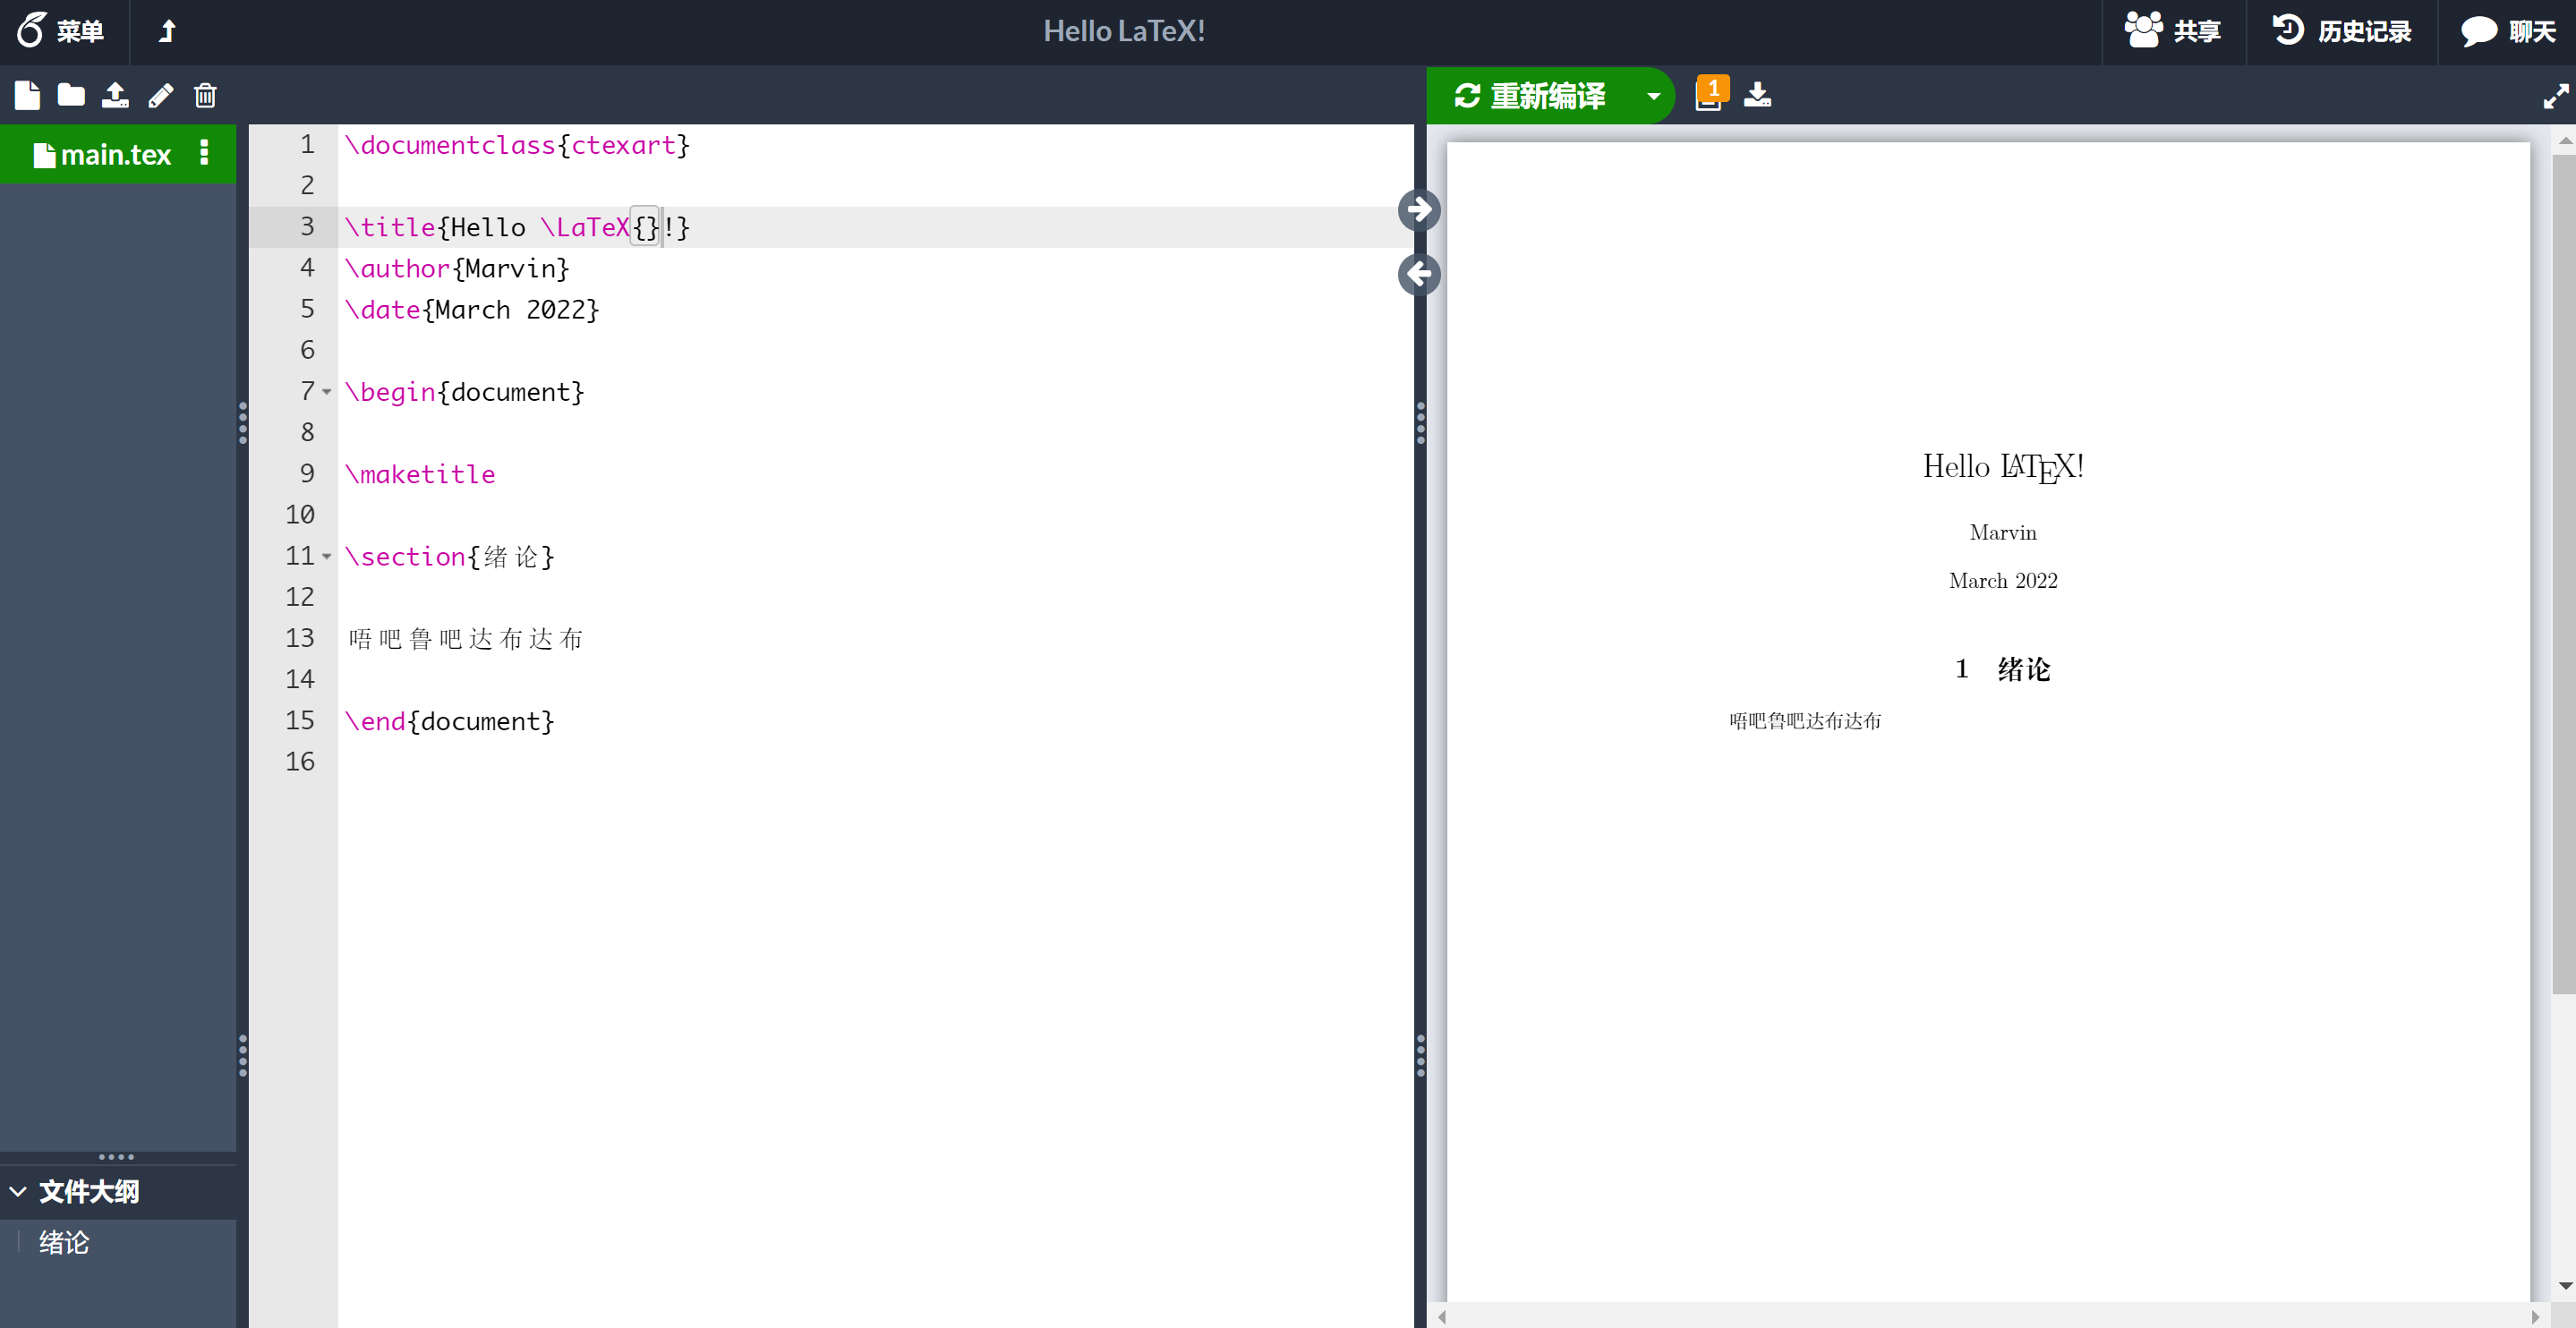
\includegraphics[width=1.3\textwidth]{nju-tex-interface}
\end{figure*}

项目创建后,得到的编辑器界面类似于图~\ref{fig:nju-tex-interface} 所示,分为源码区和预览区两大块,最左侧是文件列表。稍等片刻,预览区即会显示编译好的 PDF 文档。至此,你已经拥有了一个全功能的编译环境,可以关掉本文档去放松一下!
